\begin{table*}[t!]
\centering
\small
\begin{tabular}{@{}p{0.09\linewidth}|p{0.04\linewidth}|p{0.025\linewidth}p{0.025\linewidth}p{0.025\linewidth}p{0.025\linewidth}p{0.03\linewidth}p{0.025\linewidth}p{0.025\linewidth}p{0.025\linewidth}p{0.03\linewidth}p{0.03\linewidth}p{0.025\linewidth}p{0.03\linewidth}p{0.03\linewidth}p{0.03\linewidth}p{0.03\linewidth}p{0.03\linewidth}}
\hline
category & mean & plane & bag & cap & car & chair & ear-phone & guitar & knife & lamp & laptop & motor-bike & mug & pistol & rocket & skate-board & table \\ \hline
Wu14 \cite{wu2014interactive} & - & 63.20 & - & - & - & 73.47 & - & - & - & 74.42 & - & - & - & - & - & - & 74.76 \\
Yi16 \cite{Yi16} & 81.43 & 80.96 & 78.37 & 77.68 & \textbf{75.67} & 87.64 & 61.89 & 91.79 & 85.36 & 80.59 & 95.58 & \textbf{70.59} & 91.85 & \textbf{85.94} & 53.13 & 69.81 & 75.33 \\
ACNN \cite{boscaini2016learning} & 79.63 & 76.35 & 72.89 & 70.80 & 72.72 & 86.12 & 71.14 & 87.84 & 81.98 & 77.43 & 95.49 & 45.68 & 89.49 & 77.41 & 49.23 & 82.05 & 76.71 \\
Voxel CNN & 79.37 & 75.14 & 72.80 & 73.28 & 70.00 & 87.17 & 63.50 & 88.35 & 79.58 & 74.43 & 93.92 & 58.67 & 91.79 & 76.41 & 51.16 & 65.25 & 77.08   \\ \hline
Ours1 & 83.48 & 80.61 & 81.62 & 76.92 & 73.86 & 88.65 & 74.48 & 89.03 & 85.34 & 83.47 & 95.53 & 62.74 & 92.01 & 80.88 & \textbf{62.10} & 82.23 & 81.36 \\
Ours2 & \textbf{84.74} & \textbf{81.55} & \textbf{81.74} & \textbf{81.94} & 75.16 & \textbf{90.24} & \textbf{74.88} & \textbf{92.97} & \textbf{86.10} & \textbf{84.65} & \textbf{95.61} & 66.66 & \textbf{92.73} & 81.61 & 60.61 & \textbf{82.86} & \textbf{82.13} \\ \hline
\end{tabular}
\caption{IoU for part segmentation on 16 categories. To compute mean IoU, per category IoU is weighted by the corresponding shape number and then averaged. Ours1 represents a variation of our framework without SpecTN and Ours2 corresponds to our full pipeline with SpecTN. On average, our approach outperforms all the baseline including both traditional machine learning and deep learning based methods by a large margin. We also achieves the highest IoU on most of the categories.}
\label{tab:percatseg}
\end{table*}
\label{sec:exp}
Our proposed SyncSpecCNN takes one graph vertex function as input and predicts another as output. As a generic framework, the prediction is not limited to a specific type of graph vertex function and can be tailored towards different goals. To evaluate the effectiveness of our framework, we divide our experiments into five parts. First, we evaluate on a benchmark of 3D shape segmentation~\cite{shapenet2015,Yi16}. Second, we evaluate on keypoint prediction task using a new large scale keypoint annotation dataset. Third, we leverage SyncSpecCNN to learn vertex normal functions and visualize the prediction results qualitatively. Fourth, we perform control experiments to compare different design choices of the framework and analyze the stability of our system under input sampling density variations. Last, we show qualitative results and analyze error patterns.

\subsection{Dataset}
For 3D shape segmentation task, we use a large scale shape part annotation dataset introduced by \cite{Yi16}, which augments a subset of ShapeNet models with semantic part annotations. The dataset contains 16 categories of man-made shapes, with 2 to 6 parts per category. In total there are 16,881 models with expert verified part annotations. In addition, we use the official train/test split provided along with ShapeNet models.

For the keypoint prediction task, we build a new large scale keypoint annotation dataset, containing 1,337 chair models with 10 keypoints per shape, in contrast to traditional small scale dataset \cite{kim2013learning} which has at most 100 shapes annotated per category. These keypoints are all manually annotated by experts with consistency across different shapes. %The goal of this dataset is to allow people evaluating data-driven keypoint prediction algorithms, in contrast to traditional small scale dataset \cite{kim2013learning} which has at most 100 shapes annotated per category.

\subsection{Shape Part Segmentation} 

\myparaly{Per-category shape part segmentation}
We first conduct part segmentation assuming the category label of each shape is known, as the setting in \cite{Yi16}. The task is to predict a part label for each sample point on shapes. We compare our framework with traditional learning-based techniques \cite{wu2014interactive,Yi16} leveraging on local geometric features and shape alignment cues, as well as recent deep learning based approaches \cite{boscaini2016learning} which also fall into the family of spectral CNNs. In addition we design an additional baseline using a 3D volumetric CNN architecture, denoted as Voxel CNN, which generalizes VoxNet~\cite{maturana2015voxnet} for segmentation tasks. The network has 10 convolutional layers without down-sampling and keeps a receptive field of 19 with spatial resolution of 32. We compute per-point features in the preprocessing step as is in \cite{Yi16} and use the same set of input for all baselines except Voxel CNN. The set of input shapes are pre-aligned using a hierarchical joint alignment algorithm described in \cite{shapenet2015}. Point intersection over union (IoU) is used as evaluation metric, averaged across all part classes. Cross-entropy loss is minimized during training. 

We evaluate our framework in two settings, with or without SpecTN, and compare the results in Table~\ref{tab:percatseg}. % In practice, we find that the gain from dilation becomes marginal when SpecTN is used, even though dilation alone helps significantly. While leaving out SpecTN, 
% We used our dilated parametrization with a dilation parameter $\gamma=128$ for convolution.
%We set a dilation parameter $\gamma=128$ for convolution.

Note that on most categories our approach achieves the best performance and on average outperforms state of the art by a large margin. In comparison to \cite{boscaini2016learning},  the state of the art in the family of spectral CNNs, our approach introduces spectral dilated kernel parametrization, which increases the effectiveness of spectral CNN framework.  Moreover, the performance gain from SpecTN shows that synchronizing spectral domains would greatly increase the generalizibility across shapes of different topology and geometry. 

\iffalse
\begin{table*}[t!]
\centering
\small
\begin{tabular}{@{}p{0.04\linewidth}|p{0.05\linewidth}p{0.07\linewidth}|p{0.025\linewidth}p{0.022\linewidth}p{0.022\linewidth}p{0.022\linewidth}p{0.025\linewidth}p{0.025\linewidth}p{0.025\linewidth}p{0.025\linewidth}p{0.025\linewidth}p{0.025\linewidth}p{0.025\linewidth}p{0.025\linewidth}p{0.025\linewidth}p{0.025\linewidth}p{0.025\linewidth}p{0.025\linewidth}}
\hline
& mean partial & mean complete & plane & bag & cap & car & chair & ear-phone & guitar & knife & lamp & laptop & motor-bike & mug & pistol & rocket & skate-board & table \\ \hline
ACNN & 69.21 & 79.63 & 62.73 & 63.26 & 58.90 & 38.25 & 70.59 & \textbf{68.68} & \textbf{88.08} & 74.58 & 61.49 & 87.03 & 31.90 & 79.92 & 62.98 & 35.70 & 68.41 & 76.07 \\ \hline
Ours1 & 76.19 & 83.48 & 71.01 & 77.61 & 64.78 & 56.05 & 78.97 & 68.50 & 84.63 & 82.01 & 73.02 & 91.40 & 40.71 & 87.34 & 72.60 & \textbf{42.53} & 80.61 & 79.55 \\
Ours2 & \textbf{78.02} & \textbf{84.74} & \textbf{74.55} & \textbf{82.58} & \textbf{65.36} & \textbf{58.12} & \textbf{80.41} & 65.55 & 84.75 & \textbf{82.53} & \textbf{77.39} & \textbf{93.15} & \textbf{43.12} & \textbf{90.24} & \textbf{74.71} & 42.17 & \textbf{83.22} & \textbf{80.51} \\ \hline
\end{tabular}
\caption{IoU for part segmentation on incomplete shapes. Note that for comparison, we not only report mean IoU for partial shape part segmentation under "mean partial", but also list mean IoU for complete shape part segmentation under "mean complete". Ours1 represents a variation of our framework without SpecTN and Ours2 corresponds to our full pipeline with SpecTN. On avearge we beat ACNN, the baseline approach, by a large margin and we outperforms ACNN on most shape categories. Moreover, our approach is more robust to data incompleteness since its performance drop is lower in comparison with complete shape segmentation.}
\label{tab:partialseg}
\end{table*}
\fi

\mypara{Cross-category shape part segmentation}
Next we evaluate our approach on the part segmentation task in a cross-category setting. In this task, shape category label is not known during the test phase and for each point the network needs to select one of the part label from all possible part labels in all categories. Cross-category setting introduces larger geometric and topological variance among shapes, thus could help examining the spectral CNN's ability of recognizing objects. At the same time the impact of spectral domain misalignment becomes stronger, providing a better testbed for validating the effectiveness of SpecTN. % Essentially the network needs to have the ability to differentiate shape categories in order to do this task well. 
% Since previous supervised shape segmentation approaches mostly focus on the setting with know shape category labels, 
Since this experiment is proposed to verify design choices of spectral CNN, we mainly compare with \cite{boscaini2016learning}. We mix the 16 categories of shapes in \cite{Yi16} and train a single network for all categories. After predicting point segmentation labels, one can classify shapes through a point-wise majority voting scheme. Point IoU and classification accuracy (Acc) are chosen as the evalution metric for part segmentation and object categorization, respectively. The results are shown in the $2$nd and $3$rd column of Table~\ref{tab:partialseg}.

Our approach outperforms the baseline ACNN by a large margin on both segmentation and classification. Note that ACNN~\cite{boscaini2016learning} does not explicitly conduct multi-scale analysis and is designed for near-isometric 3D shapes with similar spectral domains, thus generalizes less well across a diverse set of shapes. Our framework, in contrast, could effectively capture multi-scale context information, a feature that is highly important for both segmentation and classification. The spectral domain synchronization ability of SpecTN  further improves our generalizability, leading to an extra performance gain as is shown in Table~\ref{tab:partialseg}.

\iffalse
\begin{table}[h!]
\centering
\begin{tabular}{@{}ccc}
\toprule
               & IoU & Classification Acc\\ \midrule
ACNN \cite{boscaini2016learning} & 69.22 & 93.99 \\
Ours without SpecTN  & 79.65 & 99.59 \\
Ours with SpecTN  & \textbf{81.97} & \textbf{99.71} \\ \bottomrule
\end{tabular}
\caption{IoU for cross category part segmentation along with an induced classification accuracy. Even without SpecTN, our approach outperforms the baseline method on both segmentation IoU and classification accuracy, due to its ability of aggregating mult-scale information. Introducing SpecTN further improves the generalizability, resulting in an extra performance gain. }
\label{tab:crosscatseg}
\end{table}
\fi

\mypara{Partial data part segmentation}
To evaluate the robustness of our approach to incomplete data, we conduct part segmentation on simulated scans of 3D shapes from a single viewpoint. To be specific, we generate $N=6$ simulated scans for each 3D shape in the part annotation dataset \cite{Yi16} from random viewpoints, and then use these partial point cloud with part annotations for train and test. All the partial point clouds are normalized to fit into a unit cube. Following the train/test split provided by \cite{shapenet2015}, we train our network to segment shape parts for each category. Again we compare our method with ACNN~\cite{boscaini2016learning}. IoU is used as evaluation metric and the results are shown in the $4$th and $5$th column of Table~\ref{tab:partialseg}.

Our approach outperforms the baseline on partial data part segmentation by a large margin. In particular, from complete shape to partial shape setting, the performance drop of our approach is less significantly than the baseline, reflected by the gap of mean IoU between the complete data setting and the partial setting. It verifies that our method is more robust to data incompleteness. We surmise that the performance of ACNN is heavily influenced by noisy and sensitive principal curvature estimation on partial scans since this step plays a crucial rule in determining its local frames; whereas our approach makes less assumption about quality of the underlying shape.

\begin{table}[t!]
\centering
\small
\begin{tabular}{@{}c|cc|cc}
\hline
& cross cat IoU & Acc & partial & complete\\ \hline
ACNN & 69.22 & 93.99 & 69.21 & 79.63 \\ \hline
Ours1 & 79.65 & 99.59 & 76.19 & 83.48 \\
Ours2 & \textbf{81.97} & \textbf{99.71} & \textbf{78.02} & \textbf{84.74} \\ \hline
\end{tabular}
\caption{The $2$nd and $3$rd column of the table reports IoU for cross category part segmentation along with an induced classification accuracy. $4$th and $5$th column of the table reports IoU for part segmentation on partial shapes and complete shapes correspondingly. Our1 and Our2 corresponds to our framework without and with SpecTN respectively. In all experiments we beat the baseline by a large margin.}
\label{tab:partialseg}
\vspace{-0.6cm}
\end{table}

\iffalse
\todo{
\begin{itemize}
    \item Per-category segmentation
        \subitem Baseline: SigAsia part annotation approach, anisotropic CNN, volumetric cnn
    \item Cross-category segmentation
        \subitem Compare our method with baseline method. show our method has the ability to do simultaneous classification and segmentation among very different graphs.
    \item Partial Data Part Segmentation
        \subitem Quantitatively and qualitatively show how our method performs on partial data. robust to missing points?
\end{itemize}
}
\fi

\subsection{Keypoint Prediction}
Our framework is not limited to part segmentation but could learn more general functions on graphs. In this section, we evaluate our framework on the keypoint prediction task. We associate each keypoint an individual label and assign all the non-keypoints a background class label. The keypoint prediction problem could be treated as a multi-class classification problem and the cross-entropy loss is optimized during training. We evaluate our approach against previous state-of-the-art method \cite{huang2013fine}. \cite{huang2013fine} first jointly aligns all the shapes in 3D space via free-form deformation and then propagates keypoint labels to test shapes from its $K$ nearest training shapes. We manually tune $K$ and report the best performance of this method. Five-folds cross validation is adopted during evaluation, and PCK (percentage of correct keypoints) is used as evaluation metric. We show the PCK curve for the two approaches in Figure~\ref{fig:keypoint}. Each point on a curve indicates fraction of correctly predicted keypoints for a given Euclidean error threshold. Our approach outperforms \cite{huang2013fine}, in particular, more precise predictions can be obtained by our method (see the region close to y-axis).

\iffalse
\todo{
We plan to manually annotate a subset of ShapeNet models and test our algorithm on supervised keypoint prediction tasks. compare with Peter's joint alignment approach.
}
\fi

\subsection{Normal Prediction}
\label{sec:normal}
To further validate the generality of our framework, we leverage our proposed SyncSpecCNN to learn another type of graph vertex function, vertex normal function. Specifically, our SyncSpecCNN takes the XYZ coordinate function of graph vertices as network input and predicts vertex normal as output. The network is trained to minimize the L2 loss between ground truth normals and predicted normals. We use the official train/test split provided by \cite{shapenet2015} and visualize some of the normal prediction results from test set in Figure~\ref{fig:normpred}.

\begin{figure}
 \centering
 \includegraphics[width=1\linewidth]{./fig/visnormal.pdf}
 \caption{We evaluate our framework on normal prediction task. The colors shown on the 3D shape are RGB-coded normals, namely putting XYZ components of normal directions into RGB channels. Our framework could predict reasonable normal directions even on very thin structures.}
 \label{fig:normpred}
\end{figure}

It can be seen our predictions are very close to the ground truth at most of the time.Even on thin structures the normal predictions are still reasonable. One problem of our prediction is that it tends to generate smoothly transiting normals along the boundary while the ground truth is sharper. This is due to the fact that we are using a small number of eigenbases in our experiments, which is not friendly to regression tasks with very high frequency signal as target.

\subsection{Diagnosis}
\myparaly{Spectral Dilated Kernel Parametrization}
 We evaluate our dilated kernel parametrization from two aspects: the basis function choice and kernel scale choice. Table~\ref{tab:kerneldesign} summarizes all the comparison results, as explained below.
 
We explore the expressive power of different kernel basis. In the family of spectral CNN, convolution kernels are parametrized by a linear combination of basis functions, i.e. modulated exponential window in our case. Previous methods have proposed to use different basis functions such as cubic spline basis \cite{bruna2013spectral} and exponential window basis \cite{boscaini2016learning}. Each row of Table~\ref{tab:kerneldesign} corresponds to a basis choice.
 
We also evaluate the effectiveness of multi-scale analysis by changing the spatial sizes of convolution kernels. We compare with two baseline choices: set all kernel size to be the smallest kernel size in the current network; set to be the largest one. Each column of Table~\ref{tab:kerneldesign} corresponds to a kernel scale choice.
 
All numbers are reported on the cross-category part segmentation task, by IoU. We only take the XYZ coordinate function of graph vertices as network input as opposed to handcrafted geometry features which may have already capture some multi-scale information. Also we remove the $7$th and $8$th layers from our network which involves SpecTN and is designed for very large convolution kernels. 

It can be seen that modulated exponential window basis has a better expressive power compared with baselines for our segmentation task. Using multi-scale kernels also enables the aggregation of multi-scale information, thus producing better performance than small or large kernels alone. 
\begin{figure}[t!]
    \centering
    \includegraphics[width=0.8\linewidth]{./fig/kpt_pred_chair.pdf}
    \caption{Keypoint prediction comparison. We draw PCK curves for both methods while changing the error threshold. Our approach outperforms \cite{huang2013fine} on average and has particularly high local accuracy when the error threshold is small, i.e. our approach reaches $pck=0.29$ when error threshold equals $0.01$, while \cite{huang2013fine} reaches $pck=0.16$}
    \label{fig:keypoint}
    \vspace{-0.5cm}
\end{figure}


\begin{table}[h!]
\centering
\small
{
\begin{tabular}{@{}lccc}
\toprule
 & small & large & multiscale \\ \midrule
Cubic Spline & 0.5369 & \multicolumn{1}{c}{-} & \multicolumn{1}{c}{-} \\
Exp Window & 0.6285 & 0.7223 & 0.7386 \\
Modulated Exp Window & 0.6997 & 0.7341 & \textbf{0.7524} \\ \bottomrule
\end{tabular}
}
\caption{We compare different kernel basis and kernel size choices, using cross category part segmentation task for evaluation. IoU is reported in the table. In particular, we compare cubic spline basis \cite{bruna2013spectral}, exponential window basis \cite{boscaini2016learning} and our modulated exponential window. All convolution kernels are parametrized by the same number of parameters and we tweak the hyper parameters of different basis functions so that their spatial sizes are comparable. We also compare three different kernel size choices. "small" indicates using small convolution kernel only; "large" indicates using large convolution kernel only; "multiscale" uses kernels of different sizes in different layers, as in our current design. It's not obvious how to parametrize multi-scale convolution kernels using cubic spline basis functions, therefore we evaluate cubic spline basis with small-sized kernels only.} 
\label{tab:kerneldesign}
\vspace{-0.3cm}
\end{table}

\paragraph{Robustness to Sampling Density Variance}
In this experiment, we evaluate the robustness of our approach w.r.t point cloud density variation. To be specific, we train our SyncSpecCNN for shape segmentation on the point cloud provided by \cite{Yi16} first. Then we downsample the point cloud under different downsample ratio and evaluate our trained model to check how segmentation performance would change. Again we evaluate our approach with/without SpecTN and the result is shown in Figure~\ref{fig:downsample}.
 
By introducing SpecTN, our framework becomes more robust to sampling density variation. Our conjecture is that sampling density variation may result in large spectral space perturbation, therefore being able to synchronize different spectral domains becomes especially important.

\begin{figure}
 \centering
 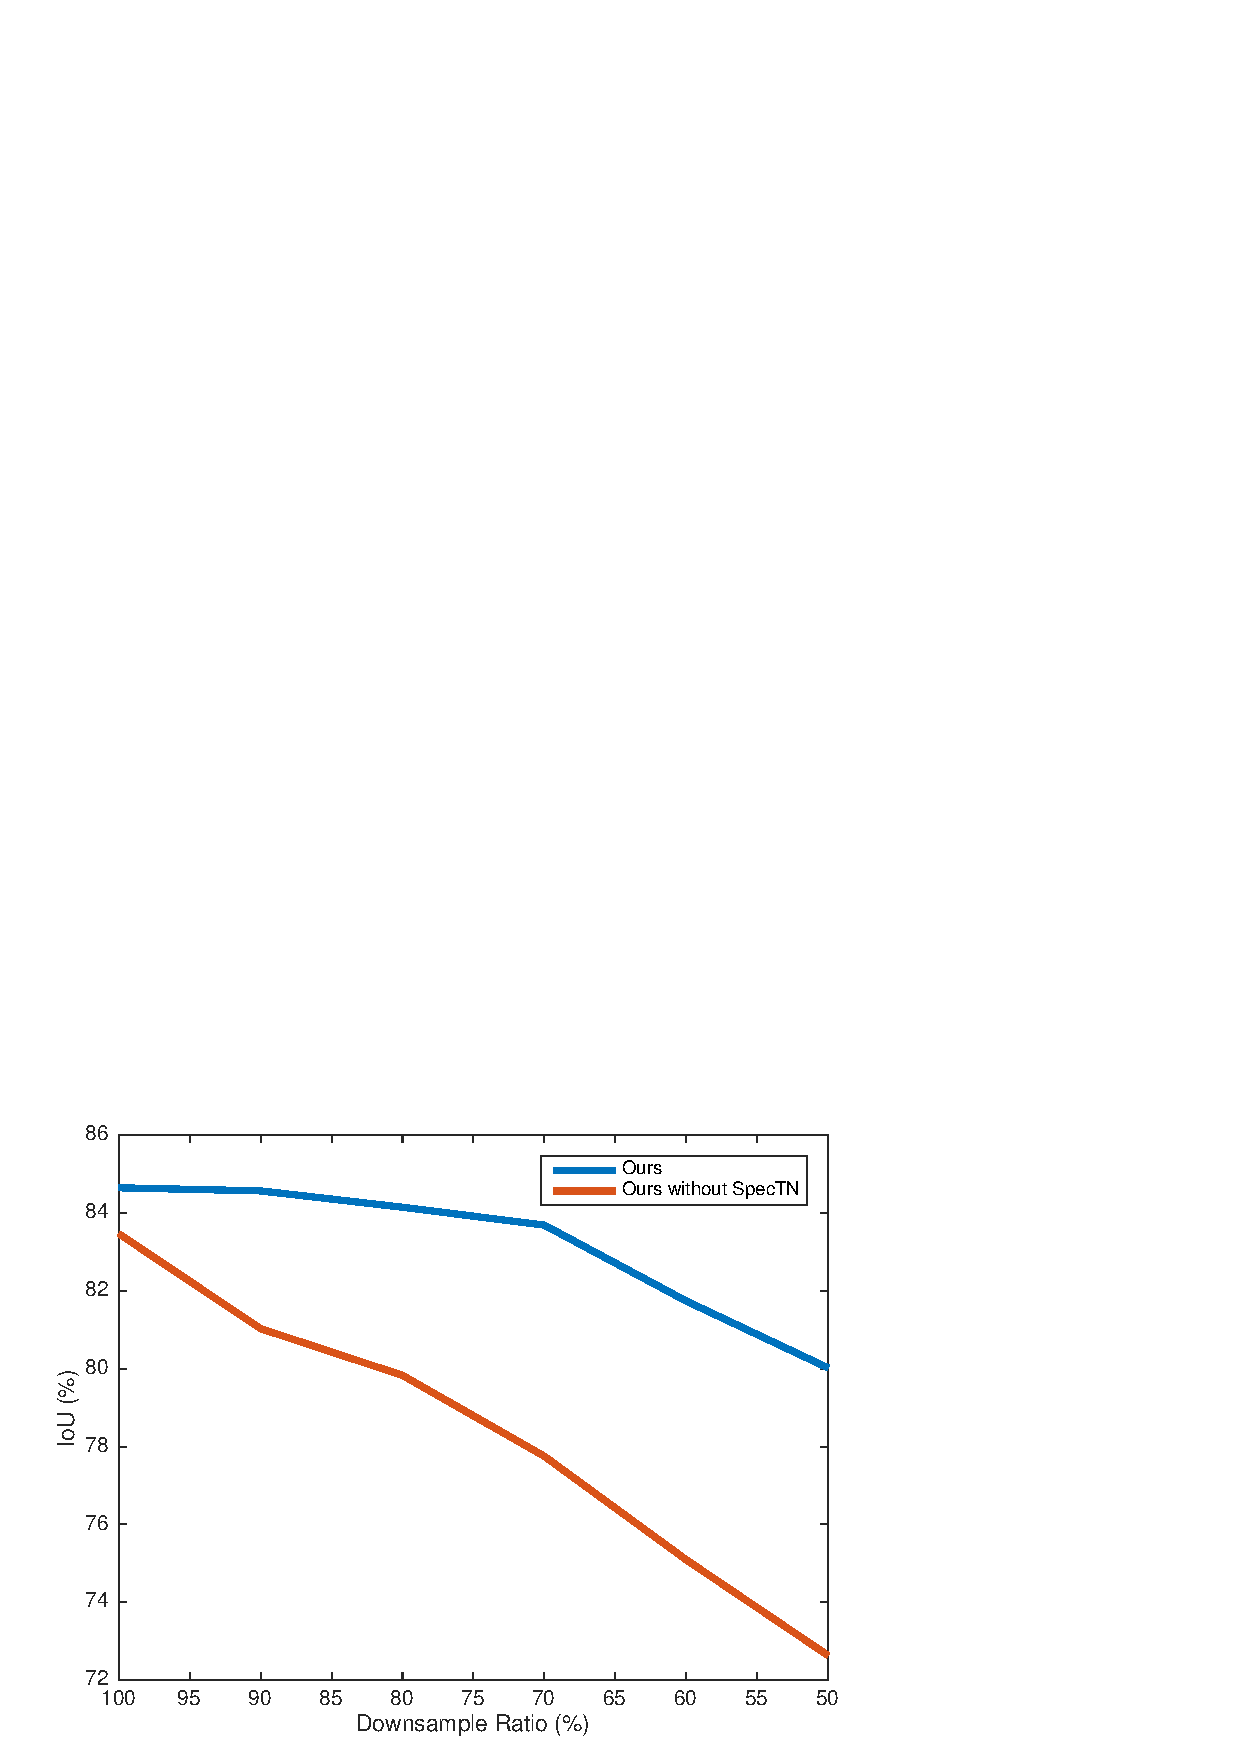
\includegraphics[width=0.8\linewidth]{./fig/downsample.pdf}
 \caption{We evaluate the robustness of our model to sampling density change. Test shapes are downsampled by different ratios and fed into our network. We compute the segmentation IoU for different downsample ratios and show it here. With SpecTN, our framework becomes more robust to sampling density change.}
 \label{fig:downsample}
\end{figure}

%\todo{Visualize joint basis}

\subsection{Qualitative Results and Error Analysis}
Figure~\ref{fig:erroranalysis} shows segmentation results generated from our network on two categories, Chair and Lamp. Representative good results are shown in the first block and  typical error patterns are summarized from the second to fourth blocks.

Most of our segmentation is very close to ground truth as is shown in the first block. We can accurately segment shapes with large geometric or topological variations like wide bench v.s. ordinary chair, pendant lamp v.s. table lamp. The lamp base on the first row and the lampshade on the second row are very similar regarding their local geometry; however, since our network is able to capture large scale context information, it could still differentiate the two and segment shapes correctly.

We observe several typical error patterns in our results. Most segmentation error occurs along part boundaries. %Our network sometimes generates fuzzy part boundaries, especially if the underlying part segments have a very smooth normal transition, as is shown in the second row of the second block. 
There are also cases where the semantic definition of parts has inherent ambiguities. %In these cases, our network may generate predictions slightly different from the ground truth but are still reasonable. 
We also observe a third type of error pattern, in which our prediction might miss a certain part completely, as is shown in the fourth block.

\begin{figure}
    \centering
    \includegraphics[width=\linewidth]{./fig/erroranalysis4.pdf}
    \caption{We visualize some segmentation results from our network prediction. The first block shows typical correct segmentations, notice the huge shape variation we can cover. The second to fourth blocks summarize different error patterns we observe in the results.}
    \label{fig:erroranalysis}
\end{figure}

\iffalse
\todo{
Compare different alternatives of our method
\begin{itemize}
    \item with multiple representatives instead of a single canonical space for spectral synchronization
    \item without join basis learning, visualize joint basis
    \item without dilated kernel, visualize dilated kernel
    \item different kernel choice: polynomial, cubic splines, exponential window, modulated exponential window
    \item different input vertex functions, extrinsic vertex functions help much since it's essentially a combination between extrinsic and intrinsic information for segmentation. intrinsic feature might not help much since the network is intrinsic and captures quite a lot intrinsic information already.
    \item network design, with/without skip link
\end{itemize}
}
\fi